\section{Понятие условного распределения случайной величины. Сформулировать определение условного ряда распределения компоненты двумерного дискретного случайного вектора. Привести рассуждения, приводящие к такому определению. Сформулировать определение условной плотности распределения компоненты двумерного непрерывного случайного вектора. Сформулировать критерии независимости случайных величин в терминах условных распределений}

\textbf{Условное распределение} случайного вектора $(X, Y)$ описывает распределение одной из случайных величин (или их совокупности) при фиксированном значении другой.

\subsubsection*{Случай дискретного случайного вектора}

Пусть выполняются следующие условия.

\begin{enumerate}
	
	\item $(X,Y)$ -- дискретный случайный вектор;
	\item $X \in \{x_1, ..., x_m\}$, $Y \in \{y_1, ..., y_n\}$;
	\item $p_{ij} = P\{(X,Y) = (x_i, y_i)\}, i = \overline{1; m}, j = \overline{1; n}$.
	
	$P_{X_i} = P\{X = x_i\}, i = \overline{1; m}$
	
	$P_{Y_j} = P\{Y = y_j\}, j = \overline{1; n}$
	
	\item Известно, что $Y = y_j$ для некоторого фиксированного $j$.
\end{enumerate}
Тогда 
\begin{align*}
	P\{X = x_i \,|\, Y = y_j\} &= 
	\left( \text{из определения условной вероятности} \right) = \\
	&= \frac{P(\{X = x_i\} \cap \{Y = y_j\})}{P(Y = y_j)} = 
	\frac{P((X, Y) = (x_i, y_j))}{P(Y = y_j)} = 
	\frac{p_{ij}}{P_Y}.
\end{align*}
Условная вероятность того, что случайная величина $Y$ приняла значение $y_j$ при условии $X = x_i$ определяется аналогично.

Набор вероятностей $P\{X = x_i \,|\, Y = y_j\}, i = \overline{1; m}$ для данного фиксированного $j$ называется условным распределением случайной величины $X$ при условии $Y = y_j$ (аналогично для случайной величины $Y$ при условии $X = x_i$ для данного фиксированного $i$). По этому набору можно составить ряд распределения, представленного таблицей значений.

\subsubsection*{Случай непрерывного случайного вектора}

В случае непрерывного случайного вектора $(X, Y)$.

Условной плотностью распределения случайной величины $X$ при условии $Y = y$ называется функция

\begin{align*}
	f_X(x|Y=y) = \frac{f(x, y)}{f_Y(y)},
\end{align*}
где $f$ -- совместная плотность распределения случайных величин $X$ и $Y$ (плотность распределения случайного вектора $(X, Y)$), $f_Y$ -- маргинальная плотность распределения случайной величины $Y$.

Аналогичным образом определяется условная плотность распределения случайной величины $Y$ при условии $X = x$.

\subsubsection*{Критерии независимости случайных величин в терминах условных распределений}

\begin{enumerate}
	
	\item Пусть $(X, Y)$ -- двумерный случайный вектор. Тогда следующие условия эквивалентны: 
	
	\begin{itemize}
		\item $X, Y$ -- независимые.
		\item $F_X(x | Y=y) \equiv F_X(x)$ для всех $y$, в которых определена $F_X(x|Y=y)$.
		\item $F_Y(y | X=x) \equiv F_Y(y)$ для всех $x$, в которых определена $F_Y(y|X=x)$.
	\end{itemize}
	\item Если $(X, Y)$ -- непрерывный случайный вектор, то следующие условия эквивалентны: 
	\begin{itemize}
		\item $X, Y$ -- независимые.
		\item $f_X(x | Y=y) \equiv f_X(x)$ для всех $y$, в которых определена $f_X(x|Y=y)$.
		\item $f_Y(y | X=x) \equiv f_Y(y)$ для всех $x$, в которых определена $f_Y(y|X=x)$.
	\end{itemize}
	\item Если $(X, Y)$ -- дискретный случайный вектор ($X \in \{x_1, ..., x_m\}$, $Y \in \{y_1, ..., y_n\}$), то следующие утверждения эквивалентны:
	\begin{itemize}
		\item $X, Y$ -- независимые.
		\item $P\{X=x_i | Y=y_j\} \equiv P\{X=x_i\}$ для всех $j=\overline{1, n}$.
		\item $P\{Y=y_j | X=x_i\} \equiv P\{Y=y_j\}$ для всех $i=\overline{1, m}$.
	\end{itemize}
\end{enumerate}


\section{Понятие функции скалярной случайной величины. Доказать теорему о формуле для вычисления плотности $f_Y(y)$ случайной величины $Y=\varphi (X)$, если $X$ – непрерывная случайная величина, а $\varphi$ –- монотонная непрерывно дифференцируемая функция. Сформулировать аналогичную теорему для кусочно-монотонной функции $\varphi$}

Пусть:
\begin{enumerate}
	\item $X$ -- некоторая случайная величина;
	\item $\varphi: \mathbb{R} \rightarrow \mathbb{R}$ -- некоторая известная функция.
\end{enumerate}

Тогда $\varphi (X) = Y$ -- некоторая случайная величина.

Если $X$ -- \textbf{непрерывная} случайная величина, то в зависимости от функции $\varphi$ случайная величина $Y = \varphi(X)$ может быть как непрерывной случайной величиной, так и дискретной или смешанного типа.

\subsection*{Теорема}

Пусть
\begin{enumerate}
	\item $X$ -- непрерывная случайная величина;
	\item $\varphi: \mathbb{R} \to \mathbb{R}$;
	\item $\varphi$ монотонна и непрерывно дифференцируема;
	\item $\psi$ -- функция, обратная к $\varphi$ (так как $\varphi$ -- монотонная, то существует $\psi = \varphi^{-1}$);
	\item $Y = \varphi(X)$.
\end{enumerate}

Тогда
\begin{enumerate}
	\item $Y$ также является непрерывной случайной величиной;
	\item Плотность вероятности $f_Y(y)$ задается следующим образом: 
	
	\begin{align*}
		f_Y(y) = f_X(\psi(y)) \cdot\left|\psi'(y)\right|.
	\end{align*}
\end{enumerate}

\subsection*{Доказательство}

\begin{enumerate}
	\item $F_Y(y) = P\{Y < y\} = P\{\varphi(X) < y\}$
	\begin{enumerate}
		\item Если $\varphi$ -- монотонно возрастающая функция, то $\varphi(X) < y \iff X < \varphi ^{-1}(y) = \psi(y)$;
		\item Если $\varphi$ -- монотонно убывающая функция, то $\varphi(X) < y \iff X > \varphi ^{-1}(y) = \psi(y)$;
	\end{enumerate}
	\item В случае случая a, $F_Y(y) = P\{X < \psi(y)\} = F_X(\psi(y))$; в случае b $F_Y(y) = P\{X > \varphi(y)\} = 1 - P\{X \preceq \psi(y)\} = \langle X \text{-- непрерывна} \rangle = 1 - P\{X < \psi(y)\} = 1 - F_X(\psi(y))$;
	\item 
	
	\[
	f_Y(y) = F_Y'(y) = 
	\begin{cases} 
		\frac{d}{dy} [F_X(\psi(y))] = F'_X(\psi(y)) \cdot \psi'(y), & \text{если a} \\
		\frac{d}{dy} [1 - F_X(\psi(y))] = -F'_X(\psi(y)) \cdot \psi'(y), & \text{если b}
	\end{cases}
	= f_X(\psi(y)) \cdot |\psi'(y)|.
	\]
	
\end{enumerate}

\subsection*{Теорема}

Пусть
\begin{enumerate}
	\item $X$ -- непрерывная случайная величина;
	\item $\varphi: \mathbb{R} \to \mathbb{R}$ является кусочно-монотонной функцией, имеющей n интервалов монотонности;
	\item $\varphi$ дифференцируема;
	\item Для данного $y \in \mathbb{R} , x_1 = x_1(y), ..., x_k = x_k(y) (k \leq n)$ -- это все решения уравнения $y = \varphi(x)$, принадлежащие интервалам $I_1, ..., I_k$ монотонности функции $\varphi$.
\end{enumerate}

Тогда для данного в последнем условии значения $y$:
\[
f_Y(y) = \sum_{j = 1}^{k} f_X (\psi_j(y)) \cdot |\psi_j'(y)|,
\]

где $\psi_j(y)$ -- функция, обратная к $\varphi(x)$ на интервале $I_j, j = \overline{1, k}$.

\section{Понятие скалярной функции случайного вектора. Обосновать формулу для вычисления функции распределения случайной величины Y , функционально зависящей от случайных величин X1 и X2, если (X1, X2) – непрерывный случайный вектор. Доказать теорему о формуле свертки}

\subsection*{Скалярные функции случайного вектора}

Пусть:
\begin{enumerate}
	\item $(X_1,X_2)$ -- двумерный случайный вектор.
	\item $\varphi: \mathbb{R}^2 \to \mathbb{R}$.
	\item $Y = \varphi(X_1, X_2)$ -- некоторая одномерная случайная величина.
\end{enumerate}

\subsection*{Случай непрерывного случайного вектора}

Если $(X_1, X_2)$ -- непрерывный случайный вектор, то функцию распределения случайной величины $Y = \varphi(X_1, X_2)$ можно найти по формуле:

\begin{align*}
	F_Y(y) = \iint\limits_{D(y)} f(x_1, x_2) \, dx_1 dx_2,
\end{align*}
где $f$ -- совместная плотность распределения случайных величин $X_1$ и $X_2$, $D(y) = \{(x_1, x_2):\varphi(x_1, x_2)<y\}$.

Пусть есть двумерный случайный вектор $(X_1, X_2)$, и:
\begin{enumerate}
	\item $(X_1, X_2)$ -- непрерывный случайный вектор;
	\item $X_1, X_2$ -- независимы;
	\item $Y = X_1 + X_2$;
	\item $f(x_1, x_2)$ -- совместная плотность распределения.
\end{enumerate}

\begin{wrapfigure}{r}{0.3\textwidth}
	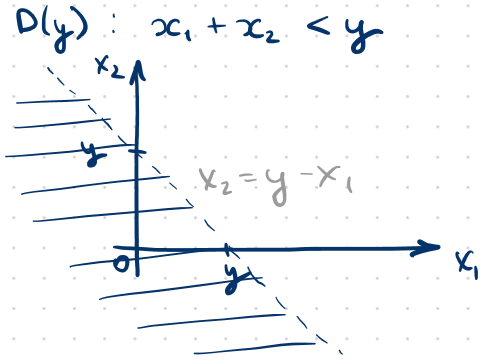
\includegraphics[width=\linewidth]{img/1.png}
\end{wrapfigure}  

Тогда $f_Y(y) = \int_{-\infty}^{+\infty} f_{X_1}(x_1)f_{X_2}(y-x_1) \, dx_1$ -- \textbf{функция свертки}.

\textbf{Доказательство}. $F_Y(y) = P\{Y<y\} = P\{X_1 + X_2 < y\} = \int \int_{D(y)} f(x_1, x_2) \, dx_1 \,dx_2 = \int_{-\infty}^{+\infty} \, dx_1 \int_{-\infty}^{y-x_1} f(x_1, x_2) \,dx_2 = \zigzagline x_1, x_2 \text{-- независимы}, f(x_1, x_2) = f_{X_1}(x_1)f_{X_2}(x_2) \zigzagline = \int_{-\infty}^{+\infty} \, dx_1 f_{X_1}(x_1) \int_{-\infty}^{y-x_1} f_{X_2}(x_2) \,dx_2 = \int_{-\infty}^{+\infty} \, dx_1 f_{X_1}(x_1) F_{X_2}(y-x_1)$. Продифференцируем: $f_Y(y) = \frac{d}{dy}(F_Y(y)) = [\int_{-\infty}^{+\infty} f_{X_1}(x_1) F_{X_2}(y-x_1) \, dx_1]' = \zigzagline \frac{d}{dy}(F_{X_2}(y-x_1)) = f_{X_2}(y-x_1) \zigzagline = \int_{-\infty}^{+\infty} f_{X_1}(x_1) f_{X_2}(y-x_1) \, dx_1$.

\section{Сформулировать определение математического ожидания для дискретной и непрерывной случайных величин. Механический смысл математического ожидания. Доказать свойства математического ожидания. Записать формулы для вычисления математического ожидания функции случайной величины и случайного вектора}

\begin{wrapfigure}{l}{0.5\textwidth}
	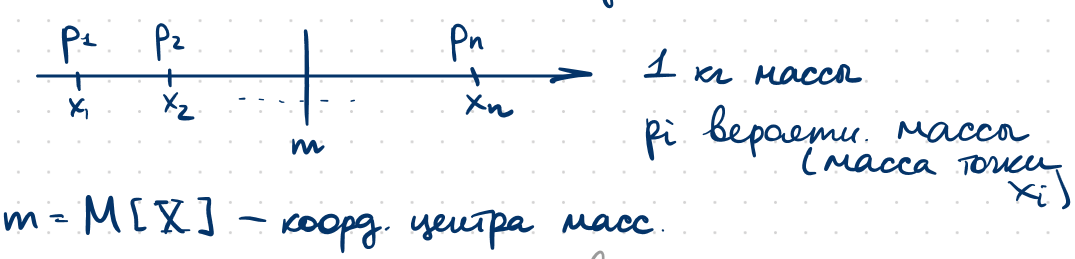
\includegraphics[width=\linewidth]{img/2.png}
\end{wrapfigure}  

Пусть $X$ -- \textbf{дискретная} случайная величина. \textbf{Математическое ожидание} (среднее значение) случайной величины $X: M[X] = \sum_{i} x_ip_i,$ где $p_i = P\{X=x_i\}$, $i$ пробегает все номера элементов конечного множества значений случайной величины.

\begin{wrapfigure}{r}{0.5\textwidth}
	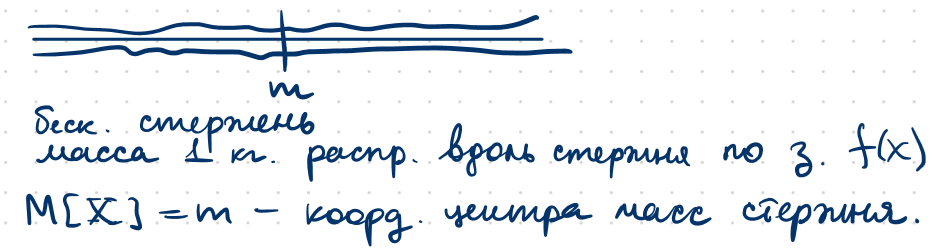
\includegraphics[width=\linewidth]{img/3.png}
\end{wrapfigure}  

Пусть $X$ -- \textbf{непрерывная} случайная величина, $f_X(x)$ -- плотность распределения. \textbf{Математическое ожидание} (среднее значение) случайной величины $X: M[X] = \int_{-\infty}^{+\infty} xf(x)\, dx$.


\textbf{Свойства}:
\begin{enumerate}
	\item Если $P\{X = x_0\} = 1$ (т.е. если $X$ фактически не является случайной), то $MX = x_0$;
	\item $M[aX + b] = a \cdot MX + b$;
	\item $M[X_1 + X_2] = MX_1 + MX_2$;
	\item Если $X_1, X_2$ -- независимы, то $M[X_1X_2] = (MX_1)(MX_2)$.
\end{enumerate}

\textbf{Доказательства}:
\begin{enumerate}
	\item Ряд распределения:
	\begin{tabular}{|>{\columncolor[gray]{0.8}}c|c|}
		\hline
		X & $x_0$ \\ \hline
		$P$ & $1$ \\ \hline
	\end{tabular}
	
	По определению: $MX = \sum_i p_ix_i = 1 \cdot x_0 = x_0$;
	
	\item Докажем для случая непрерывной случайной величины:
	
	\begin{align}
		M[aX + b] &= \langle \varphi(x) = ax + b; aX + b \text{ -- непрерывная случайная величина} \rangle \notag \\
		&= \int_{-\infty}^{+\infty} (ax+b)f(x) \, dx = a \int_{-\infty}^{+\infty} x f(x) \, dx + b \int_{-\infty}^{+\infty} f(x) \, dx \notag \\
		&= a \cdot MX + b \notag;
	\end{align}
	
	\item Доказательство для дискретного случая. Элементы $X_1$ обозначаются индексами $i$, пробегающими множество $I$; для $X_2$ используются $j$ и $J$. Запись о:
	
	\begin{align}
		M[X_1 + X_2] &= \langle \varphi(x_1, x_2) = x_1 + x_2 \rangle \notag \\
		&= \sum_{i \in I} \sum_{j \in J} (x_{1, i} + x_{2, j})p_{ij} =  \sum_{i \in I} \sum_{j \in J} x_{1, i}p_{ij} +  \sum_{i \in I} \sum_{j \in J} x_{2, j}p_{ij} \notag \\
		&= \sum_{i \in I} x_{1, i} \sum_{j \in J} p_{ij} + \sum_{j \in J} x_{2, j} \sum_{i \in I} p_{ij} \notag \\
		&= MX_1 + MX_2 \notag;
	\end{align}
	
	\item Докажем для непрерывных случайных величин:
	
	\begin{align}
		M[X_1X_2] &= \langle \varphi(x_1, x_2) x_1x_2 \rangle = \int \int_{R^2} x_1x_2f(x_1, x_2) \, dx_1 \, dx_2 \notag \\
		&= \langle X_1, X_2 \text{ -- независимы} \Rightarrow f(x_1, x_2) = f_{X_1}(x_1)f_{X_2}(x_2) \rangle \notag \\
		&= \int_{-\infty}^{+\infty} \, dx_1 \int_{-\infty}^{+\infty} x_1x_2f_{X_1}(x_1)f_{X_2}(x_2) \, dx_2 = (\int_{-\infty}^{+\infty} x_1f_{X_1}(x_1) \, dx_1) (\int_{-\infty}^{+\infty} x_2f_{X_2}(x_2) \, dx_2) \notag \\
		&= (MX_1) (MX_2) \notag.
	\end{align}
	
\end{enumerate}

\subsection*{Формулы для вычисления математического ожидания}

\begin{enumerate}
	\item $X$ -- случайная величина, $\varphi: \mathbb{R} \rightarrow \mathbb{R}$:
	\begin{itemize}
		\item $M[\varphi(X)] = \sum_{i} \varphi(x_i)p_i$, если $X$ -- дискретная случайная величина;
		\item}$M[\varphi(X)] = \int_{-\infty}^{+\infty} \varphi(x)f(x) \, dx$, если $X$ -- непрерывная случайная величина, $f(x)$ -- плотность;
\end{itemize}
\item $\vec{X} = (X_1, X_2)$ -- случайный вектор, $\varphi: \mathbb{R}^2 \rightarrow \mathbb{R}, Y = \varphi(X_1, X_2)$. $p_{ij} = P_i\{(X_1, X_2) = (x_{1, i}, x_{2, j})\}$:
\begin{itemize}
	\item $M[\varphi(X_1, X_2)] = \sum_{i, j} \varphi (x_{1, i}, x_{2, j})p_{ij}$, если $\vec{X}$ -- дискретный вектор;
	\item $M[\varphi(X_1, X_2)] = \int_{-\infty}^{+\infty} \int_{-\infty}^{+\infty} \varphi(x_1, x_2)f(x_1, x_2) \, dx_1 \, dx_2$, где $f(x_1, x_2)$ -- совместная плотность непрерывного случайного вектора $\vec{X}$.
\end{itemize}
\end{enumerate}


\section{Сформулировать определение дисперсии случайной величины. Механический смысл дисперсии. Доказать свойства дисперсии. Понятие среднеквадратичного отклонения случайной величины}

\textbf{Дисперсией} случайной величины $X$ называется $DX = M[(X-m)^2],$ где $m=MX$.

Если $X$ -- \textbf{дискретная} случайная величина, то $DX = \sum_{i} (x_i - m)^2 p_i$, где $p_i = P\{X=x_i\}$. Если  $X$ -- \textbf{непрерывная} случайная величина, то $DX = \int_{-\infty}^{+\infty} (x-m)^2f(x) \, dx$, где $f$ -- функция плотности случайной величины $X$.

\textbf{Механический смысл дисперсии:} дисперсия является моментом инерции вероятностной массы относительно точки $m=MX$, т.е. характеризует <<разброс>> вероятностной массы относительно математического ожидания этой случайной величины. Чем больше $D$, тем больше <<разброс>>.

\textbf{Свойства}:
\begin{enumerate}
	\item для любого случайного вектора $X: DX \geq 0$;
	\item если $P\{X=x_0\} = 1,$ то $DX = 0$;
	\item $D[aX+b] = a^2DX,      a, b = const$;
	\item $D[X] = M[X^2] - (MX)^2$;
	\item если $X_1, X_2$ -- независимые случайные величины, то $D[X_1 + X_2] = D[X_1] + D[X_2]$.
\end{enumerate}

\textbf{Доказательства}:
\begin{enumerate}
	\item $DX = MY$, где $Y = (X - m)^2$. Т.к. $Y \geq 0$, то следует, что $DX = MY \geq 0$;
	\item ...
	\begin{tabular}{|>{\columncolor[gray]{0.8}}c|c|}
		\hline
		X & $x_0$ \\ \hline
		$P$ & $1$ \\ \hline
	\end{tabular}
	
	Математическое ожидание $MX = m = x_0$. Дисперсия $DX = \sum_{i} (x_i - m)^2p_i = (x_0 = x_0)^2 \cdot 1 = 0$;	
	\item
	
	\begin{align}
		D[aX + b] &= M[[(aX+b) - M(aX+b)]^2] = M[[aX + b - a \cdot MX - b]^2]  \notag \\
		&= M[(a(X-MX))^2] = a^2M[(X -MX)^2] \notag \\
		&= a^2DX \notag;
	\end{align}
	
	\item Обозначим $m = MX$, тогда:
	\begin{align}
		DX &= M[(X=m)^2] = M[X^2-2mX +m^2] = M[X^2]-2m\cdot M[X]+m^2 \notag \\
		&= M[X^2]-m^2 \notag;
	\end{align}
	
	\item 
	\begin{align}
		D(X_1 + X_2) &= \langle \text{по свойству 4} \rangle = M[(X_1 + X_2)^2] - (M(X_1 + X_2))^2 \notag \\
		&= M[X_1^2] + M[X_2^2] + 2M[X_1X_2] - (MX_1)^2 - (MX_2)^2 - 2MX_1 \cdot MX_2 = \notag \\
		&=  \langle X_2, X_2 \text{ -- независимые, тогда } M[X_1X_2] = MX_1 \cdot MX_2 \rangle \notag \\
		&= (M[X_1^2] - (MX_1)^2) + (M[X_2^2] - (MX_2)^2) \notag \\
		&= DX_1 + DX_2 \notag.
	\end{align}
	
\end{enumerate}

$DX$ имеет размерность, равную квадрату размерности случайной величины $X$. Это не всегда удобно на практике, поэтому рассматривают такую числовую характеристику, как среднеквадратичное отклонение.

\textbf{Среднеквадратичным отклонением} случайной величины $X$ называют число $\sigma_X = \sqrt{D[X]}$. 

\section{Сформулировать определение математического ожидания и дисперсии. Записать законы распределения биномиальной, пуассоновской, равномерной, экспоненциальной и нормальной случайной величин. Найти математические ожидания и дисперсии этих случайных величин}

Пусть $X$ -- \textbf{дискретная} случайная величина. \textbf{Математическое ожидание} (среднее значение) случайной величины $X: M[X] = \sum_{i} x_ip_i,$ где $p_i = P\{X=x_i\}$, $i$ пробегает все номера элементов конечного множества значений случайной величины.

Пусть $X$ -- \textbf{непрерывная} случайная величина, $f_X(x)$ -- плотность распределения. \textbf{Математическое ожидание} (среднее значение) случайной величины $X: M[X] = \int_{-\infty}^{+\infty} xf(x)\, dx$.

\textbf{Дисперсией} случайной величины $X$ называется $DX = M[(X-m)^2],$ где $m=MX$.

\subsection*{Биноминальная случайная величина}

Говорят, что случайная величина $X$ имеет биноминальное распределение с параметром $n \in \mathbb{N}$ и $p \in (0, 1)$, если она принимает значения $0, 1, ..., n$ с вероятностями: $P\{X = k\} = C_n^k \cdot p^k \cdot q^{n-k}, k = \overline{0, n}, q = 1 - p.$ Обозначается: $X \sim B(n, p)$.

\[
MX = M[\sum_{i = 1}^{n} X_i] = \sum_{i = 1}^{n} MX_i = np
\]

\[
DX = D[\sum_{i = 1}^{n} X_i] = \langle X_i \text{ независимы } \rangle = \sum_{i = 1}^{n} DX_i = npq.
\]

\subsection*{Пуассоновская случайная величина}

Говорят, что случайная величина $X$ распределена по закону Пуассона с параметром $\lambda > 0$, если она принимает значения $0, 1, 2, ...$ с вероятностями: $P\{X = k\} = \frac{\lambda ^ k}{k!}\cdot e^{-\lambda}, k \in \{0, 1, 2, ...\}$. Обозначается: $X \sim \text{П}(\lambda)$.

\begin{align}
	MX &= \sum_{k = 0}^{\infty} k \frac{\lambda^k}{k!} e^{-\lambda} = e^{-\lambda} \sum_{k=1}^{\infty}k \frac{\lambda^k}{k!} = e^{-\lambda} \sum_{k=1}^{\infty} \frac{\lambda^{k-1} \lambda}{(k-1)!} \notag \\
	&= \lambda e^{-\lambda} \sum_{k=1}^{\infty} \frac{\lambda^{k-1}}{(k-1)!} = \langle i = k -1 \rangle = \lambda e^{-\lambda} \sum_{i=0}^{\infty} \frac{\lambda^i}{i!} \notag \\
	&= \lambda \notag.
\end{align}

Дисперсия выражается как $DX = M[X^2] - (MX)^2$.

\[
MX^2 = \sum_{k = 0}^{\infty} k^2 \frac{\lambda^k}{k!} e^{-\lambda} = ... = \lambda^2 + \lambda. \text{ Тогда } DX = \lambda.
\].


\subsection*{Равномерное распределение}

Говорят, что случайная величина $X$ имеет равномерное распределение на отрезке $[a, b]$, если она является непрерывной случайной величиной с функций плотности распределения: 

\[
f(x) = 
\begin{cases} 
	c, & x \in [a, b] \\
	0, & \text{иначе}
\end{cases}
, \text{где } c = const.
\]

Обозначается: $X \sim R(a, b)$.

$X \sim R(0, 1)$.

\[
f(x) = 
\begin{cases} 
	\frac{1}{b-a}, & x \in (a, b) \\
	0, & \text{иначе}
\end{cases}
\]

\[
MX = \int_{-\infty}^{\infty} xf(x) \, dx = \frac{1}{b-a} \int_a^b x \, dx = \frac{1}{2(b-a)}(b^2-a^2) = \frac{a+b}{2}
\]

\begin{align}
	DX &= \int_{-\infty}^{+\infty} (x-\frac{a+b}{2}) f(x) \, dx = \frac{1}{b-a} \int_a^b (x-\frac{a+b}{2})^2 \, dx \notag \\
	&= \frac{1}{3(b-a)}(x-\frac{a+b}{2})^3 \left| \substack{a \\ \\ \\ b} \right = \frac{1}{3(b-a)} (\frac{(b-a)^3}{8} - \frac{(a-b)^3}{8}) = \frac{(b-a)^3}{12(b-a)} \notag \\
	&= \frac{(b-a)^2}{12} \notag.
\end{align}

\subsection*{Экспоненциальное распределение}

Говорят, что случайная величина $X$ распределена по закону с параметром $\lambda > 0$, если $X$ является непрерывной случайной величиной, функция плотности которой имеет вид:

\[
f(x) = 
\begin{cases} 
	\lambda e^{-\lambda x}, & x \geq 0 \\
	0, & \text{иначе.}
\end{cases}
\]

Обозначается: $X \sim Exp(\lambda)$.

\begin{align}
	MX &= \int_{-\infty}^{+\infty} xf(x)x = \lambda \int_{0}^{+\infty} xe^{-\lambda x} \, dx = -\int_{0}^{+\infty} x \, de^{-\lambda x} \notag \\
	&= -xe^{-\lambda x} \left| \substack{+\infty \\ \\ \\ 0} \right + \int_{0}^{+\infty} e^{-\lambda x} \, dx = -\frac{1}{\lambda} e^{-\lambda x} \left| \substack{+\infty \\ \\ \\ 0} \right \notag \\
	&= \frac{1}{\lambda} \notag.
\end{align}

$DX = M[X^2] - (MX)^2$,

\begin{align}
	M[X^2] &= \int_{-\infty}^{+\infty} x^2 f(x) \, dx = \lambda \int_{0}^{+\infty} x^2 e^{-\lambda x} \, dx = -\int_{0}^{+\infty} x^2 \, de^{-\lambda x} = -x^2e^{-\lambda x} \left| \substack{+\infty \\ \\ \\ 0} \right + 2 \int_{0}^{+\infty} xe^{-\lambda x} \, dx \notag \\
	&= \frac{2}{\lambda^2} \notag.
\end{align}

Таким образом, $DX = \frac{2}{\lambda^2} - (\frac{1}{\lambda})^2 = \frac{1}{\lambda^2}$.

\subsection*{Нормальное распределение}

Говорят, что случайная величина $X$ имеет нормальное распределение с параметрами $m$ и $\sigma ^2$, если $X$ -- является непрерывной случайной величиной, функция плотности которой имеет вид:

\[
f(x) =  \frac{1}{\sqrt{2 \pi} \cdot \sigma} \cdot e^{-\frac{(x-m)^2}{2\sigma ^2}}, x \in \mathbb{R}.
\]

Обозначается: $X \sim N(m, \sigma ^2)$.

\begin{align}
	MX &= \int_{-\infty}^{+\infty} xf(x) \, dx = \frac{1}{\sigma \sqrt{2 \pi}} \int_{-\infty}^{+\infty} xe^{-\frac{(x-m)^2}{2 \sigma^2}} \, dx = \langle x-m= t \rangle \notag \\
		&= \frac{1}{\sigma \sqrt{2 \pi}} \int_{-\infty}^{+\infty} (t+m) e^{-\frac{t^2}{2\sigma^2}} \, dt =  \frac{1}{\sigma \sqrt{2 \pi}} \int_{-\infty}^{+\infty} te^{-\frac{t^2}{2\sigma^2}} \, dt + m \cdot  \frac{1}{\sigma \sqrt{2 \pi}} \int_{-\infty}^{+\infty} e^{-\frac{t^2}{2\sigma^2}} \, dt \notag \\
		&= m.
\end{align}

\begin{align}
	DX &= M[(X-MX)^2] = \int_{-\infty}^{+\infty} (x-m)^2 f(x) \, dx = \frac{1}{\sigma \sqrt{2 \pi}} \int_{-\infty}^{+\infty} (x-m)^2e^{-\frac{(x-m)^2}{2 \sigma^2}} \, dx \notag \\
	&= \langle \frac{x-m}{\sigma} = t, dx = \sigma \, dt \rangle = \frac{\sigma^2}{\sqrt{2 \pi}} \int_{-\infty}^{+\infty} t^2 e^{-\frac{t^2}{2}} \, dt =\frac{\sigma^2}{2\sqrt{2 \pi}} \int_{-\infty}^{+\infty} te^{\frac{t^2}{2}} \, dt^2 \notag \\
	&= - \frac{\sigma^2}{\sqrt{2 \pi}} \int_{-\infty}^{+\infty} t \, de^{-\frac{t^2}{2}} \, dt^2 = \langle \text{ по частям } \rangle = -\frac{\sigma^2}{\sqrt{2 \pi}} te^{-e\frac{t^2}{2}}  \left| \substack{+\infty \\ \\ \\ - \infty} \right + \sigma^2 \cdot \frac{1}{\sqrt{2 \pi}} \int_{-\infty}^{+\infty} e^{-\frac{t^2}{2}} \, dt \notag \\
	&= \sigma^2.
\end{align}

\section{Сформулировать определение ковариации и записать формулы для ее вычисления в случае дискретного и непрерывного случайных векторов. Доказать свойства ковариации}

Ковариация является числовой характиристикой случайного вектора. Пусть $(X_1, X_2)$ -- двумерный случайный вектор. $Ковариацией$ случайной величины $X_1$ и $X_2$ называется число $cov(X_1, X_2) = M[(X_1 - m_1)(X_2 - m_2)],$ где $m_i = MX_i, i = \overline{1, 2}$.

Если $X_1, X_2$ - дискретный случайные величины, то $cov(X_1, X_2) = \sum_{i_1, i_2}(x_{1, i_1}-m_1)(x_{2, i_2}-m_2)p_{i_1i_2},$ где $p_{i_1i_2} = P\{(X_1, X_2) = (x_{1, i_1}, x_{2, i_2})\}$.

Если $X_1, X_2$ - непрерывные случайные величины, то $cov(X_1, X_2) = \int \int_{\mathbb{R}} (x_1 - m_1)(x_2 - m_2) f(x_1, x_2) \, dx_1 \,dx_2$, где $f$ -- совместная плотность распределения $X_1$ и $X_2$.

\textbf{Свойства}:
\begin{enumerate}
	\item $D[X+Y] = DX + DY + 2cov(X, Y)$;
	\item $cov(X, X) = DX$;
	\item если $X, Y$ -- независимы, то $cov(X, Y) = 0.$ Обратное не верно;
	\item $cov(a_1X + b_1, a_2Y + b_2) = a_1a_2cov(X, Y)$;
	\item $|cov(X, Y)| \leq \sqrt{DX \cdot DY}$, причем $|cov(X, Y)| = \sqrt{DX \cdot DY} \equiv$ случайные величины $X$ и $Y$ связаны линейной зависимостью;
	\item $cov(X, Y) = M[XY] - (MX)(MY)$.
\end{enumerate}

\textbf{Доказательства}:
\begin{enumerate}
	\item 
	\begin{align}
		D(X+Y) &= M[((X+Y) - M[X+Y])^2] = \langle MX = m_1, MY = m_2 \rangle = M[((X-m_1) - M[Y-m_2])^2] \notag \\ 
		&= M[(X-m_1)^2] + M[(Y-m_2)^2] + 2M[(X-m_1)(Y-m_2)] = \notag \\
		&= DX + DY + 2cov(X, Y) \notag;
	\end{align}
	
	\item $cov(X, X) = M[(X-m)(X-m)] = M[(X-m)^2] = DX$;
	\item 
	\begin{align}
		cov(X, Y) &= M[(X-m_1)(Y-m_2)] = \langle X, Y \text{ -- независимые } \Rightarrow \notag \\
		& (X-m_1) \text{ и } (Y-m_2) \text{ тоже независимые } \rangle = [M(X-m_1)][M(Y-m_2)] \notag \\ 
		&= 0\notag;
	\end{align}
	
	\item 
	\begin{align}
		cov(a_1X + b_1, a_2X + b_2) &=  M[[a_1X + b_1 - M(a_1X + b_1)] \cdot [a_2X+b_2-M(a_2X + b_2)]] \notag \\ 
		&= M[[a_1X + b_1 - a_1m_1 -b_1][a_2X+b_2 -a_2m_2 - b_2]] \notag \\
		&= M[a_1a_2(X_1-MX_1)(X_2 - MX_2)] \notag;
	\end{align}
	
	\item
	\begin{enumerate}
		\item Выберем произвольное число $t \in \mathbb{R}$. Рассмотрим случайную величину $Z(t) = tX - Y$. Тогда $D[Z(t)] = D[tX - Y] = \langle \text{ свойство 1 + свойство дисперсии } \rangle = t^2DX + DY - 2t \cdot cov(X, Y) = DX \cdot t^2 - 2t \cdot cov(X, Y) + DY \text{ -- квадратный трехчлен относительно } t$. Так как $D[X(t)] \geq 0$, следовательно, трехчлен должен быть параболой вверх, т.е. дискриминант $D \leq 0$.
		
		\[
		\frac{D}{4} = (cov(X, Y))^2 - DX \cdot DY \leq 0 \Rightarrow |cov(X, Y)| \leq \sqrt{DX \cdot DY};
		\]	
		
		\item Необходимость ($\Rightarrow$). Если $|cov(X, Y)| = \sqrt{DX \cdot DY} \Rightarrow$ дискриминант $=0 \Rightarrow D[Z(t)]$ имеет единственный корень. Обозначим его $t = a \Rightarrow Z(a) = aX - Y$ принимает единственное значение с вероятностью 1, обозначим это значение как $-b \Rightarrow Z(a) = aX - Y = -b \Rightarrow Y=aX+b$; 
		\item Достаточность ($\Leftarrow$). Если $Y = aX + b \Rightarrow Z(a) = -b \Rightarrow D[Z(a)] = 0 \Rightarrow$ дискриминант $= 0 \Rightarrow |cov(X, Y)| = \sqrt{DX \cdot DY}$.
	\end{enumerate}
	
	\item
	\begin{align}
		cov(X, Y) &=  M[(X - m_1)(Y-m_2)] = M[XY - m_1Y - m_2X + m_1m_2] \notag \\
		&= M[XY] - m_1MY - m_2MX + m_1m_2 \notag \\
		&= M[XY] - m_1m_2 \notag;
	\end{align}
	
\end{enumerate}

\section{Сформулировать определение ковариации и коэффициента корреляции случайных величин. Сформулировать свойства коэффициента корреляции. Сформулировать определения независимых и некоррелированных случайных величин, указать связь между этими свойствами. Понятия ковариационной и корреляционной матриц. Записать свойства ковариационной матрицы}

Ковариация является числовой характиристикой случайного вектора. Пусть $(X_1, X_2)$ -- двумерный случайный вектор. $Ковариацией$ случайной величины $X_1$ и $X_2$ называется число $cov(X_1, X_2) = M[(X_1 - m_1)(X_2 - m_2)],$ где $m_i = MX_i, i = \overline{1, 2}$.

Недостатком ковариации является то, что она имеет размерность равную произведению разностей случайных величин $X$ и $Y$. Часто рассматривают аналогичную безразмерную характеристику, которая называется коэффициентом корреляции случайных величин $X$ и $Y$:

\[
\rho(X, Y) = \rho_{XY} = \frac{cov(X, Y)}{\sqrt{DX \cdot DY}},
\] 
где $DX \cdot DY > 0$.

\textbf{Свойства коэффициента корреляции}:
\begin{enumerate}
	\item $\rho_{XX} = 1$;
	\item Если $X, Y$ -- независимые, то $\rho_{XY} = 0$;
	\item $\rho(a_1X + b_1, a_2Y + b_2) \pm \rho(X, Y),$ причем $\pm$ заменяется на
	\begin{itemize}
		\item $+$, если $a_1a_2 < 0$;
		\item $-$, если $a_1a_2 > 0$;
	\end{itemize}
	\item $\rho_{XY} \leq 1$, причем:
	\[
	\rho_{XY} =
	\begin{cases} 
		1, & \text{когда } Y = aX + b, \text{где } a > 0 \\
		-1, & \text{когда } Y = aX + b, \text{где } a < 0
	\end{cases}
	\]
\end{enumerate}

Случайные величины $X$ и $Y$ называются некоррелированными, если $cov(X, Y) = 0$.

\(F(x, y) = F_X(x) F_Y(y)\), где \( F \) -- совместная функция распределения \( X \) и \( Y \) ($\equiv$ функция распределения случайного вектора \( (X, Y) \)); \( F_X \), \( F_Y \) -- маргинальные функции распределения случайных величин \( X \) и \( Y \).

Из свойства 3 ковариации следует, что еслим $X, Y$ -- независимые, то $X, Y$ -- некоррелированные. Обратное неверно.

\textbf{Ковариационной матрицей} случайного вектора $\vec{X}$ называется матрица

\[
\sum_{\vec{X}} = (\sigma_{ij})_{i, j = \overline{1, n}},
\]

где $\sigma_{ij} = cov(X_i, X_j)$.

\textbf{Свойства коэффициента корреляции}:
\begin{enumerate}
	\item $\sigma_{ii} = DX_i$;
	\item $\sum_{\vec{X}} = \sum_{\vec{X}}^{T}$;
	\item Если $\vec{Y} = \vec{X}B + \vec{c}$, где $\vec{Y} = (Y_1, ..., Y_m), \vec{X} = (X_1, ..., X_n), B \in M_{n, m}(\mathbb{R})$ (т.е. $\vec{Y}$ является линейной функцией от вектора $\vec{X}$), то $\sum_{\vec{Y}} = B^T \sum_{\vec{X}} B$;
	\item Матрица $\sum_{\vec{X}$ является неотрицательной определенной, т.е. $\forall \vec{b} \in \mathbb{R}^w: \vec{b}^T \sum_{\vec{X}} \vec{b} \geq 0$;
	\item Если все компоненты вектора $\vec{X}$ попарно независимы, то $\sum_{\vec{X}$ -- диагональная матрица.
\end{enumerate}

\textbf{Корреляционной матрицей} вектора $\vec{X} = (X_1, ..., X_n) называют матрицу$

\[
P = (\rho_{ij})_{i, j = \overline{1, n}}, 
\]

где $\rho_{ij} =\rho(X_i, X_j)$.


\section{Понятие условного распределения компоненты двумерного случайного вектора (дискретный и непрерывный случаи). Сформулировать определения значений условного математического ожидания и условной дисперсии. Сформулировать определения условного математического ожидания и условной дисперсии. Записать формулы для вычисления условных математического ожидания и дисперсии для компоненты двумерного нормального вектора}

a

\section{Понятие n-мерного нормального распределения. Сформулировать основные свойства многомерного нормального распределения}

a